\chapter{O jogo do triângulo amoroso}

Vimos que a assimetria de informação pode levar o jogo a um resultado que não é ótimo para nenhum dos jogadores, onde um jogador é capaz de, até mesmo, aumentar seu pagamento ao mudar de estratégia unilateralmente. Porém em jogos iterados o jogo eventualmente evoluirá para os hiper-equilíbrios do sistema, pois os jogadores são capazes de identificar explorar as hiper-preferências dos demais. Esse comportamento pode ser observado no jogo do triângulo amoroso, que iremos definir a seguir.

Neste jogo temos três jogadores em um grafo completo, um triângulo no qual todos interagem entre si, onde todos jogadores são amigos, porém existem sentimentos não correspondidos que mudam a forma como eles interagem. Para ilustrar essa dinâmica vamos considerar duas estratégias, $\textit{cozinhar}$ e $\textit{lavar a louça}$, ou $C$ e $L$. Consideramos que cada um possui sua própria matriz de pagamentos, definidas abaixo. Lembre-se que a entrada $b_{k,i,j}$ da matriz $B_k$ é o pagamento do jogador $k$ ao usar a estratégia $i$ contra a estratégia $j$, com $k\in\{u,v,w\}$ e $i,j\in\{C,L\}$, neste caso.

\begin{equation}
    \label{payoffLoveTri}
    B_u=
    \begin{bmatrix}
        0 & 1\\ 
        0 & 0 
    \end{bmatrix},
    B_v=
    \begin{bmatrix}
        0 & 0\\ 
        1 & 0 
    \end{bmatrix},
    B_w=
    \begin{bmatrix}
        1 & 0\\ 
        0 & 0 
    \end{bmatrix}
\end{equation}

Note que $u$ e $v$ se complementam, pois $u$ só possui pagamento ao $\textit{cozinhar}$ (jogar a estratégia $C$) para alguém que vá $\textit{lavar a louça}$ (jogar a estratégia $L$) e $v$ só possui pagamento ao $\textit{lavar a louça}$ para alguém que vá $\textit{cozinhar}$, enquanto $w$ só se beneficia ao $\textit{cozinhar}$ junto com o outro (jogar a estratégia $C$ para $C$). Assim, com jogadores racionais, é esperado que o perfil $(e_1,e_2,e_1)$ seja o resultado final do jogo, onde $u$ e $v$ irão se relacionar de maneira complementar, $v$ receberá um pagamento de ambas suas relações e $w$ irá conseguir algum benefício apenas de sua relação com $u$.

Este jogo se torna interessante ao considerarmos jogadores hiper-racionais, pois as interações entre eles deixam de ser tão óbvias. Considere o caso no qual o jogador $u$ possui sentimentos por $v$, $v$ possui sentimentos por $w$ que, por sua vez, possui somente amor próprio. Essas relações podem ser representadas através da seguinte matriz de preferências.
\begin{equation}
    \label{prefPosLoveTri1}
    \Rc=
    \begin{bmatrix}
        \frac{1}{2} & \frac{1}{2} & 0\\ 
        0 & \frac{3}{5} & \frac{2}{5} \\
        0 & 0 & 1
    \end{bmatrix}
\end{equation}

Assim, as equações de replicação de cada jogador serão como segue.

\begin{equation}
    \label{EqRepLoveTri1}
    \left\{\begin{matrix*}[l]
        \dot{x}_{u,C}=x_{u,C}(1-x_{u,C})\left(\frac{3}{4}x_{v,L}+\frac{1}{4}x_{w,L}\right) \\
        \dot{x}_{v,C}=x_{v,C}(1-x_{v,C})\left(-\frac{3}{10}x_{u,C}-\frac{1}{10}x_{w,C}\right) \\
        \dot{x}_{w,C}=x_{w,C}(1-x_{w,C})\left(\frac{1}{2}x_{u,C}+\frac{1}{2}x_{v,C}\right)
    \end{matrix*}\right.
\end{equation}

Pelas equações, podemos concluir que o resultado será o mesmo do jogo clássico, o perfil de estratégias $(e_1,e_2,e_1)$. Isso pode ser observado na figura \ref{fig:love_tri1.png}.

\begin{figure}[h]
    \caption{Evolução do uso da estratégia $C$ para cada jogador do triângulo amoroso com $\Rc$ dada em $\eqref{prefPosLoveTri1}$,  $[0.5 \; 0.5]^T$ como condição inicial para todos jogadores e $t\in[0,40]$.}
    \centerline{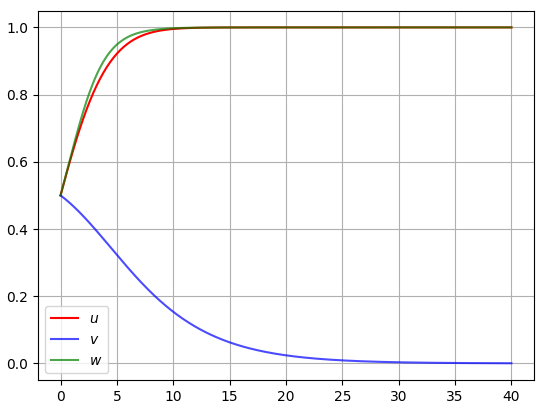
\includegraphics[scale=0.8]{./img/love_tri1.png}}
    \label{fig:love_tri1.png}
\end{figure}

Para tornar o jogo mais interessante vamos supor que $v$ esteja cada vez mais apaixonado por $w$ e passe a valorizá-lo com a mesma intensidade que valoriza a si mesmo. Por conta disso, $u$ começa a desconfiar dos sentimentos de $v$ e, por ciúmes, passa a querer o prejuízo de $w$. Essa nova dinâmica pode ser representada pela seguinte matriz de preferências.

\begin{equation}
    \label{prefPosLoveTri2}
    \Rc=
    \begin{bmatrix}
        \frac{2}{5} & \frac{2}{5} & -\frac{1}{5}\\ 
        0 & \frac{1}{2} & \frac{1}{2} \\
        0 & 0 & 1
    \end{bmatrix}
\end{equation}

Com essas mudanças, as equações $\eqref{EqRepLoveTri1}$ serão dadas por
\begin{equation}
    \label{EqRepLoveTri2}
    \left\{\begin{matrix*}[l]
        \dot{x}_{u,C}=x_{u,C}(1-x_{u,C})\left(\frac{2}{5}x_{v,L}+\frac{1}{5}x_{w,L} -\frac{1}{10}x_{w,C}\right) \\
        \dot{x}_{v,C}=x_{v,C}(1-x_{v,C})\left(\frac{1}{4}x_{w,C}-\frac{1}{4}x_{u,C}\right) \\
        \dot{x}_{w,C}=x_{w,C}(1-x_{w,C})\left(\frac{1}{2}x_{u,C}+\frac{1}{2}x_{v,C}\right)
    \end{matrix*}\right.
\end{equation}

Note que a equação de $w$ não mudou e, portanto, se $x_{u,C}>0$ ou $x_{v,C}>0$ teremos que $x_{w,C}\to 1$. Então, assumindo que $x_{w,C}=1$ enquanto $x_{u,C},x_{v,C}\in(0,1)$ para algum $t>0$ , temos que
\begin{equation}
    \label{uDedicav}
    \dot{x}_{u,C}>0 \Longleftrightarrow x_{v,C} \leq \frac{3}{4},
\end{equation}
ou seja, uma condição para que $u$ continue jogando $C$ e agradando ao jogador $v$. Porém, ao mesmo tempo, temos
\begin{equation}
    \label{vDedicau}
    \dot{x}_{v,C} \leq 0 \Longleftrightarrow x_{u,C} \geq x_{w,C},
\end{equation}
que nos dá uma condição para que $v$ não deixe de jogar $L$, que agrada o jogador $u$, para jogar $C$, que agrada o jogador $w$. Caso as condições $\eqref{uDedicav}$ e $\eqref{vDedicau}$ não sejam satisfeitas, teremos como solução o perfil de estratégias $(e_2,e_1,e_1)$, onde $u$ passa a jogar $L$ apenas para diminuir o pagamento de $w$, pois ele não recebe mais nenhum benefício de sua relação com $v$, que agora joga $C$ para aumentar o pagamento de $w$ mesmo não recebendo nenhum pagamento efetivo dessa relação. Essa dinâmica pode ser observada na figura \ref{fig:love_tri2.png}.

\begin{figure}[h]
    \caption{Evolução do uso da estratégia $C$ para cada jogador do triângulo amoroso com $\Rc$ dada em $\eqref{prefPosLoveTri2}$,  $[0.5 \; 0.5]^T$ como condição inicial para todos jogadores e $t\in[0,120]$.}
    \centerline{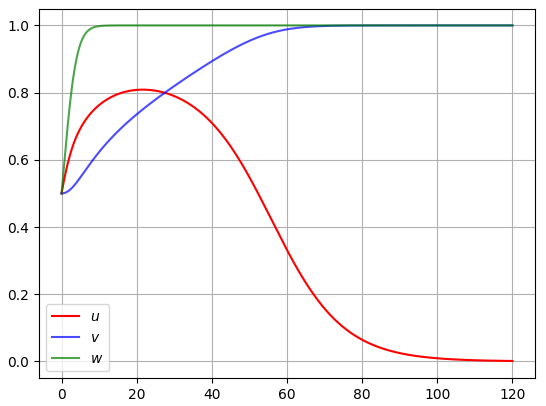
\includegraphics[scale=0.8]{./img/love_tri2.png}}
    \label{fig:love_tri2.png}
\end{figure}

Apesar de parecer simples, essa dinâmica de $\textit{cozinhar}$ e $\textit{lavar a louça}$ pode se tornar complicada quando inserimos os sentimentos humanos como variáveis. Neste exemplo conseguimos modelar afeição e ciúmes através das hiper-preferências dos jogadores, exemplificando o que foi dito no capítulo \ref{chap:hiperRacionalidade} e mostrando como a hipótese de racionalidade não é suficiente para modelar o comportamento humano em todas situações.